\documentclass[11pt,twocolumn]{article}

\usepackage{epsfig}
\usepackage{graphicx}
\usepackage{graphpap}
\usepackage{amsmath}
\usepackage[utf8]{inputenc}
\usepackage[spanish]{babel}

\topmargin -2.5 cm
\textheight 9.5in
\oddsidemargin -1cm
%\evensidemargin -1cm
\textwidth 18cm
%opening
\title{}
\author{}
\date{}

\newcommand{\abre}{\textquestiondown}

\begin{document}

\pagestyle{empty}
\sffamily
\twocolumn[
Física de campos. TALLER 3: \textbf{Campo y potencial eléctrico }

\hrulefill 
\vspace{0.5 cm}
]
\footnote{Las figuras han sido tomadas en su gran mayora de Physics For Scientist and Engineers 6E By Serway and Jewett.}

\begin{enumerate}
%ejercicio
\item Una barra cargada de longitud $l$ tiene una carga positiva por unidad de longitud $\lambda$ y una carga total $Q$. Calcule el campo eléctrico $\vec{E}$ y el potencial eléctrico en un punto $P$ a lo largo del eje de la barra a una distancia $a$ de uno de los extremos.
{
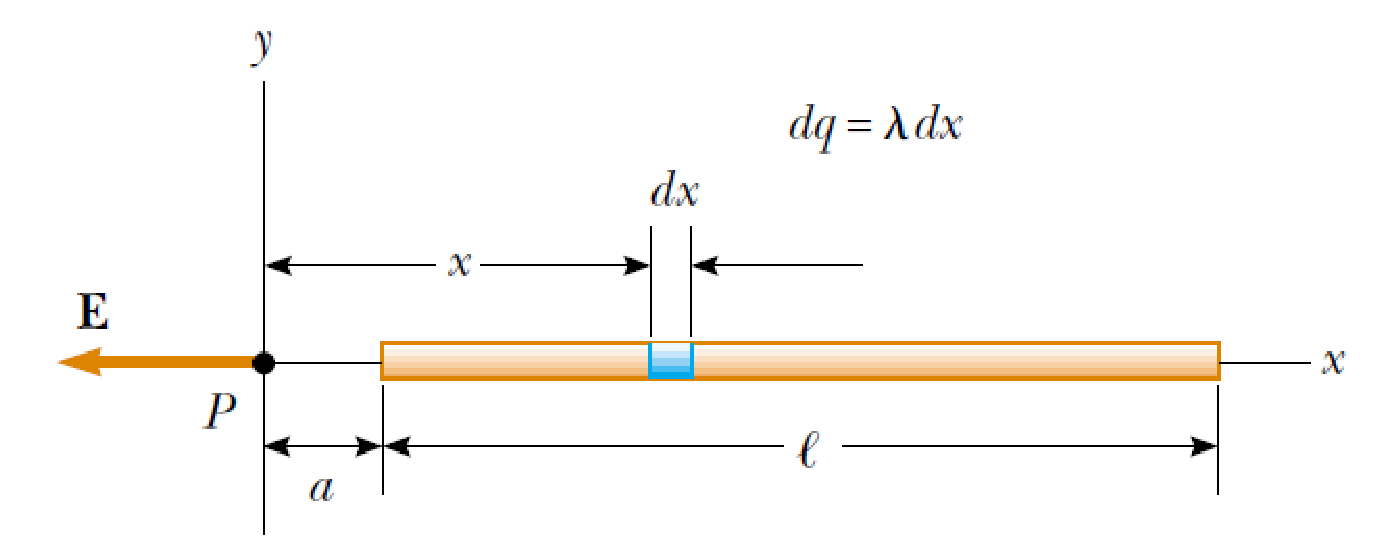
\includegraphics[scale=0.3]{barra}
}
\begin{displaymath}
\vec{E}=-\dfrac{kQ}{a(a+l)} \hat{i}
\end{displaymath}
\small{Note que para $a\gg l$ la barra se comporta como una carga puntual.} 

%ejercicio
\item Un anillo de radio $R$ tiene una carga positiva $Q$ uniformemente distribuida. Calcule el campo y el potencial eléctrico a una distancia $x$ a lo largo del eje del anillo.
{
\begin{center}
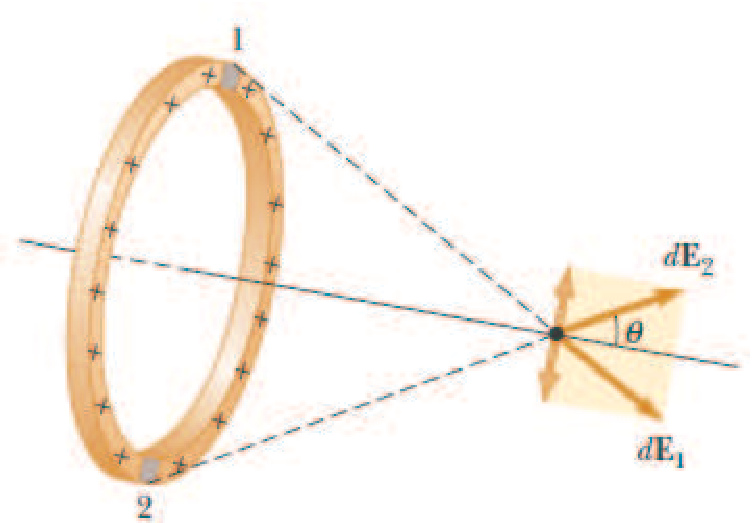
\includegraphics[scale=0.3]{anillo}
\end{center}
}
\begin{displaymath}
\vec{E}=\dfrac{kQ x}{(R^2+x^2)^{3/2}} \hat{i} \hspace{0.7 cm} V=\dfrac{kQ}{\sqrt{x^2 +R^2}}
\end{displaymath}
\small{Note que para $x\gg R$ el anillo se comporta como una carga puntual $Q$.} 

%ejercicio
\item Un disco de radio $R$ tiene una carga uniforme por unidad de área $\sigma$. Calcule el campo y el potencial eléctrico a lo largo del eje del disco a una distancia $x$ de su centro.
{
\begin{center}
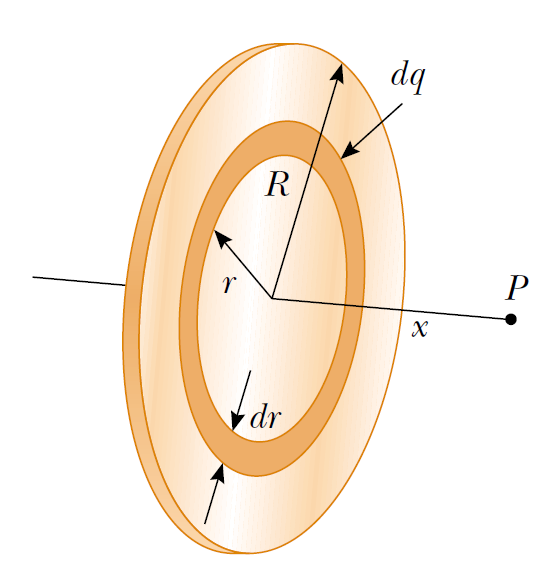
\includegraphics[scale=0.2]{disco}
\end{center}
}
\begin{displaymath}
\vec{E}=2\pi k \sigma \Big(1-\dfrac{x}{(x^2+R^2)^{3/2}}\Big)\hat{i}
\end{displaymath}
\small{Note que para $x\gg a$ el disco se comporta como una carga puntual $Q$.} 

%ejercicio
\item Una esfera \textit{aislante} de radio $a$ tiene una carga $Q$ distribuida uniformemente. 
\begin{enumerate}
\item Calcule el campo y el potencial eléctrico en un punto interno ($r \leq a$).  
\item Calcule el campo y el potencial eléctrico en un punto externo ($r\geq a$).  
\end{enumerate}
{
\begin{center}
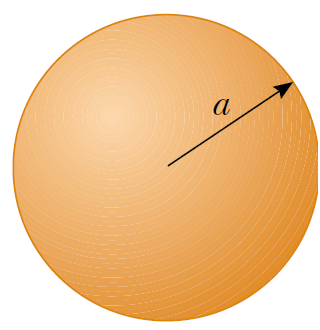
\includegraphics[scale=0.2]{esfera}
\end{center}
}
\begin{displaymath}
\vec{E}=k\dfrac{Q}{r^2}\hat{u_{r}} \hspace{0.2 cm} (r \geq a) \hspace{0.6 cm} \vec{E}=k\dfrac{Q r}{a^3}\hat{u_{r}} \hspace{0.2 cm} (r \leq a)
\end{displaymath}
\begin{displaymath}
V=k\dfrac{Q}{r} \hspace{0.2 cm} (r\geq a) \hspace{0.6 cm} V=\dfrac{kQ}{2a}\Big(3-\dfrac{r^2}{a^2}\Big) \hspace{0.2 cm} (r\leq a)
\end{displaymath}

%ejercicio
\item Una esfera \textit{conductora} de radio $a$ tiene una carga $Q$. 
\begin{enumerate}
\item Calcule el campo y el potencial eléctrico en un punto interno ($r\leq a$).  
\item Calcule el campo y el potencial eléctrico en un punto externo ($r\geq a$).  
\end{enumerate}
{
\begin{center}
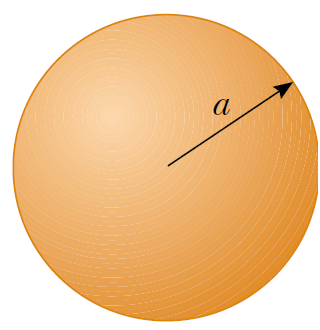
\includegraphics[scale=0.2]{esfera}
\end{center}
}
\begin{displaymath}
\vec{E}=k\dfrac{Q}{r^2}\hat{u_{r}} \hspace{0.2 cm} (r \geq a) \hspace{0.6 cm} E=0 \hspace{0.2 cm} (r \leq a)
\end{displaymath}
\begin{displaymath}
V=k\dfrac{Q}{r} \hspace{0.2 cm} (r\geq a) \hspace{0.6 cm} V=\dfrac{kQ}{a} \hspace{0.2 cm} (r\leq a)
\end{displaymath}

%ejercicio
\item Considere un disco hueco de radio exterior $R_{1}$ e interior $R_{2}$ y carga $Q$ uniformemente distribuida. 
\begin{enumerate}
\item Halle el campo y el potencial eléctrico en un punto $P$ a lo largo del eje del disco.
\begin{displaymath}
\vec{E}=\dfrac{2kQ}{(R_{1}^2 -R_{2}^2)}\Big[\dfrac{z}{\sqrt{R_{1}^2 +z^2}}- \dfrac{z}{\sqrt{R_{2}^2 +z^2}}\Big]\hat{k}
\end{displaymath}
\begin{displaymath}
V= \dfrac{2kQ}{(R_{1}^2 -R_{2}^2)}\Big[\sqrt{R_{1}^2 + z^2} - \sqrt{R_{2}^2 +z^2}\Big]
\end{displaymath}
\item Analize el caso cuando $R_{1} \to 0$ (dese cuenta que en ese caso se tiene un disco). Analize el caso cuando $R_{1} \to 0$ y $R_{2} \to \infty $ (dese cuenta que en este caso se tiene un plano infinito).
\end{enumerate}

%ejercicio
\item Considere dos barras uniformes de longitud $l$ y carga $Q$ colocadas a lo largo de la misma línea y que tienen sus puntos más cercanos separados una distancia $d$. Muestre que la fuerza eléctrica mutua entre las dos barras es:
\begin{displaymath}
F_{e}= k\dfrac{Q^2}{l^2} \ln \Big[\dfrac{(l+d)^2}{d(2l+d)}\Big]
\end{displaymath}  

%ejercicio
\item Una varilla de carga $Q$ es doblada en forma de semicírculo de radio $R$. Calcule el campo y el potencial eléctrico en el centro del semicírculo.
\begin{displaymath}
\vec{E}=\dfrac{2kQ}{\pi}\dfrac{1}{R^2} \hat{j} \hspace{1.0 cm} V=\cdots
\end{displaymath} 
{
\begin{center}
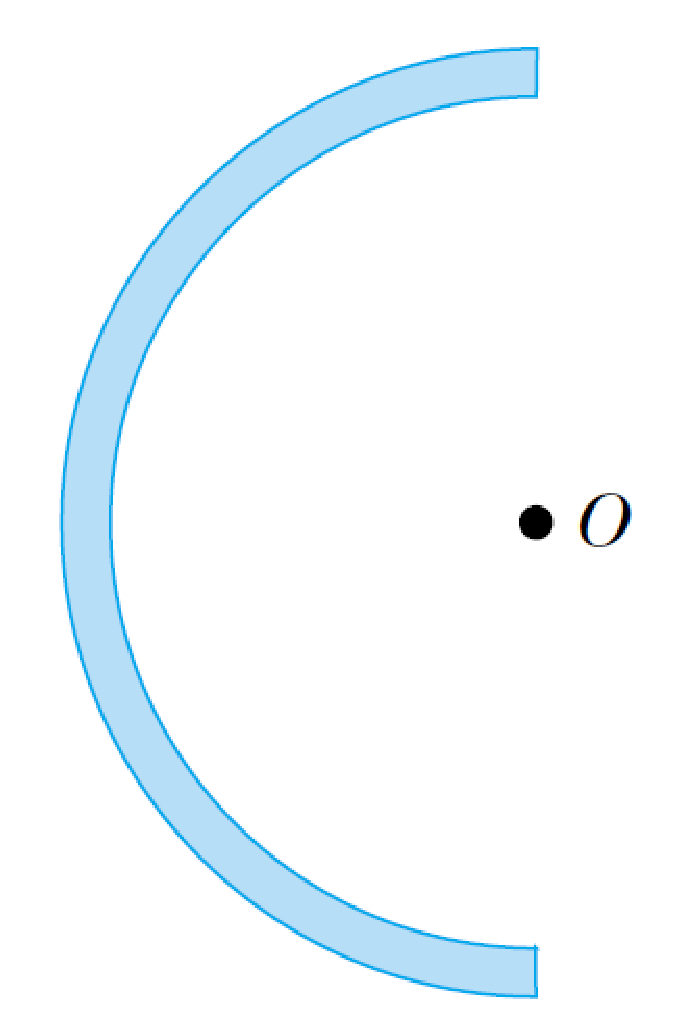
\includegraphics[scale=0.15]{media-barilla}
\end{center}
}

%ejercicio 9
\item Calcule el campo y el potencial eléctrico de una varilla finita de longitud $l$ y densidad de carga $\lambda$ a lo largo de un eje perpendicular a la varilla y que pase por el centro de la misma.
\begin{displaymath}
E=\dfrac{k\lambda}{y}\dfrac{l}{\sqrt{l^2/4+y^2}} \hspace{0.3 cm} 
V=k\lambda \ln\left(\dfrac{\sqrt{l^2/4+y^2}+l/2}{\sqrt{l^2/4+y^2}-l/2}\right)
\end{displaymath}
{
\begin{center}
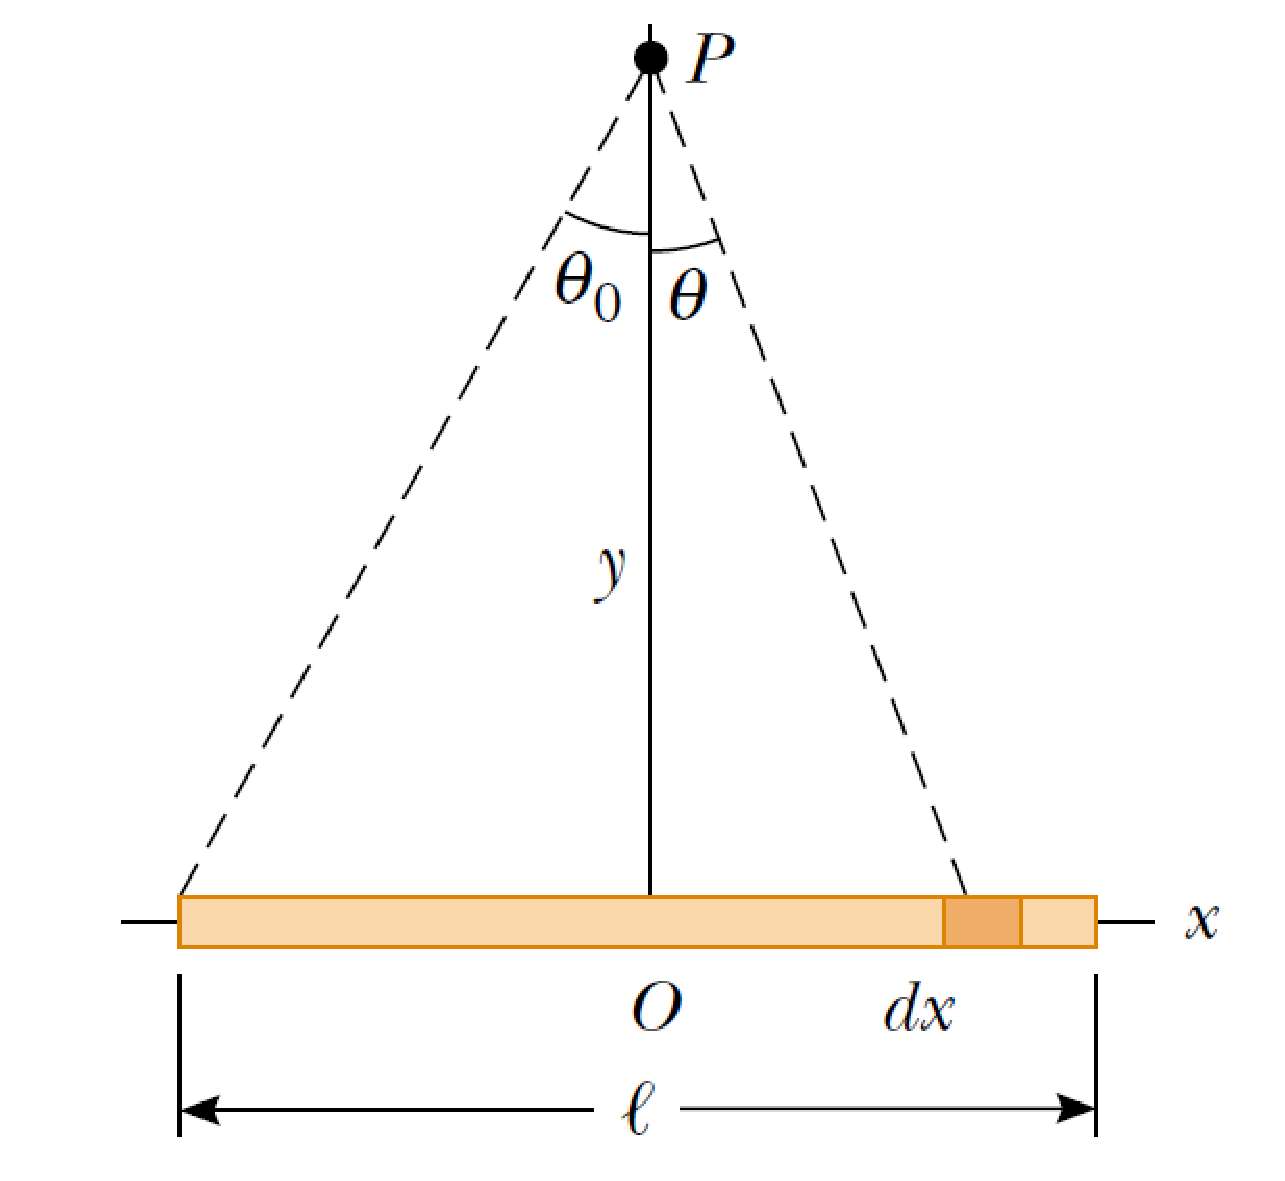
\includegraphics[scale=0.2]{varilla-finita}
\end{center}
}

%ejercicio 10
\item Calcule el campo y el potencial eléctrico de una varilla infinita de densidad de carga $\lambda$.
\begin{displaymath}
\vec{E}=\dfrac{2k\lambda}{r}\hat{u_{r}} \hspace{1.0 cm} V=-2k\lambda \ln(y)
\end{displaymath}

%ejercicio 
\item Un dipolo eléctrico es colocado en un campo eléctrico uniforme tal como se muestra en la figura. En ella se ve que el dipolo está desplazado ligeramente de su posición de equilibrio ($\theta$ pequeño). La separación de las cargas es $2a$ y el momento de inercia del dipolo a lo largo de un eje perpendicular que pase por el punto medio de la línea de separación de las dos cargas es $I$. Muestre que dicho dipolo tiene un M.A.S. con frecuencia angular de oscilación $f$.
\begin{displaymath}
f=\dfrac{1}{2\pi}\sqrt{\dfrac{2qaE}{I}}
\end{displaymath}   
{
\begin{center}
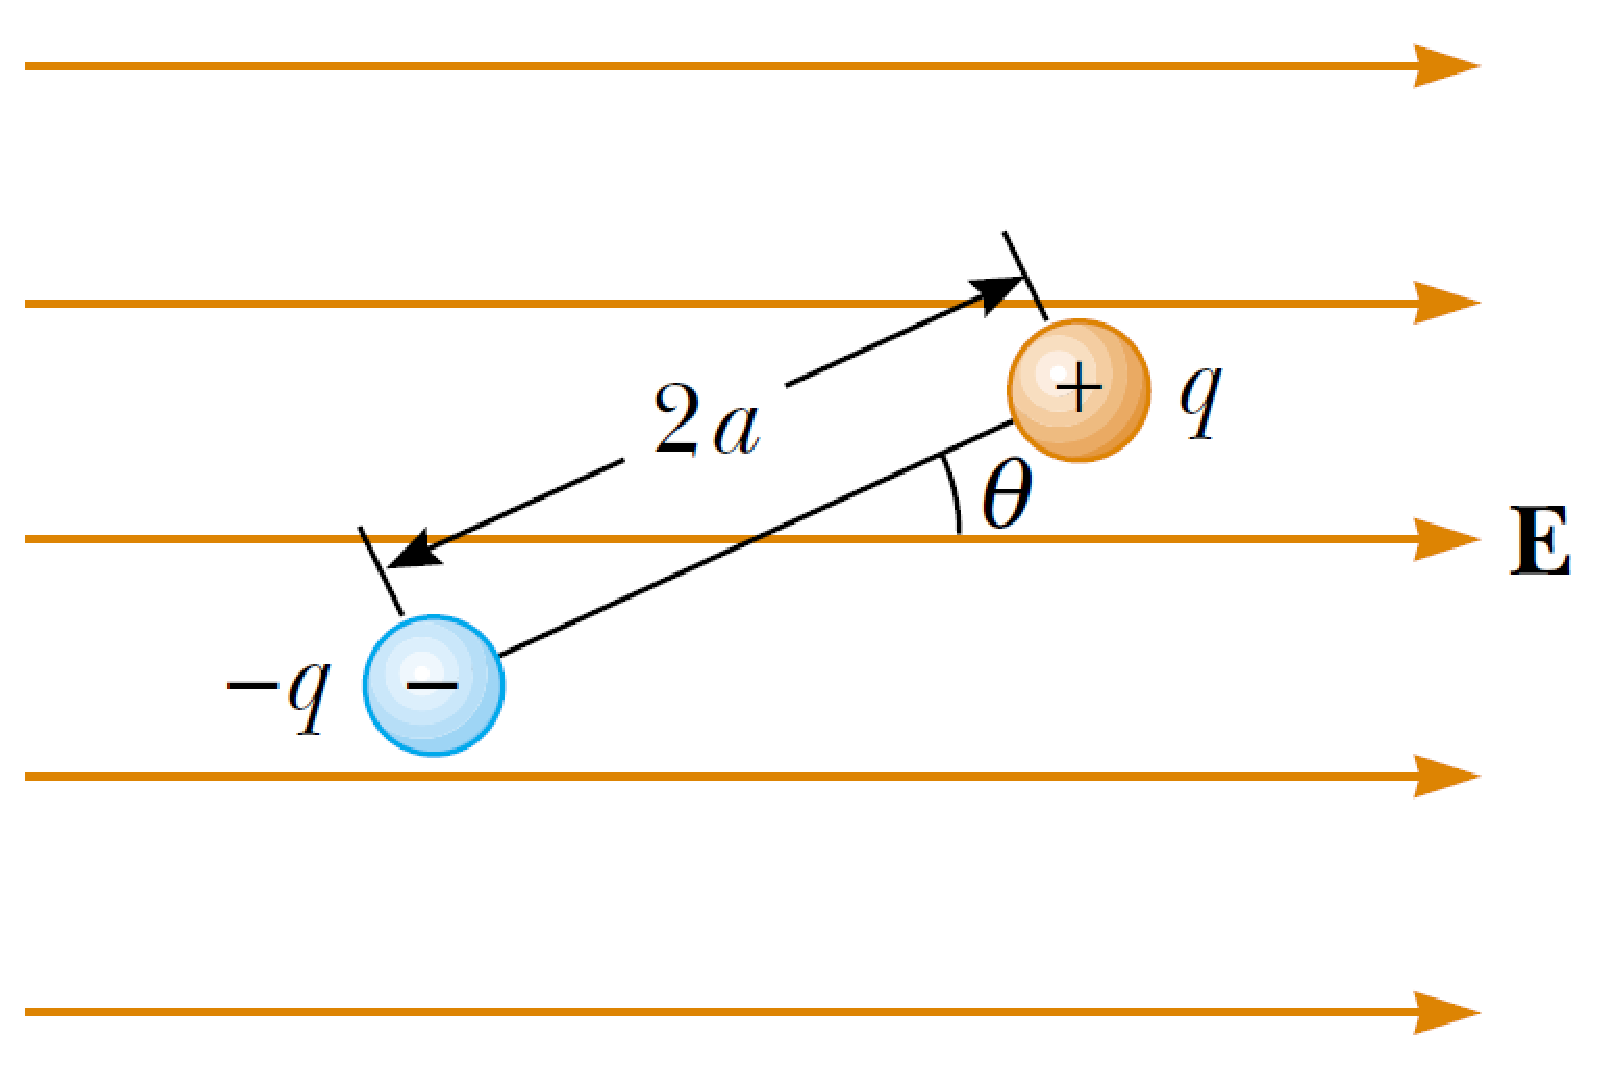
\includegraphics[scale=0.2]{MAS-dipolo}
\end{center}
}

%ejercicio
\item Calcule el campo y el potencial eléctrico de un plano infinito de densidad de carga superficial $+\sigma$.
\begin{displaymath}
\vec{E}=\dfrac{\sigma}{2\epsilon_{0}}\hat{k} \hspace{1.0 cm} V=-\dfrac{\sigma}{2\epsilon_{0}}z
\end{displaymath}

%ejercicio
\item Calcule el campo eléctrico de un par de placas paralelas (infinitas) de densidad de carga $\sigma$ y $-\sigma$.
{
\begin{center}
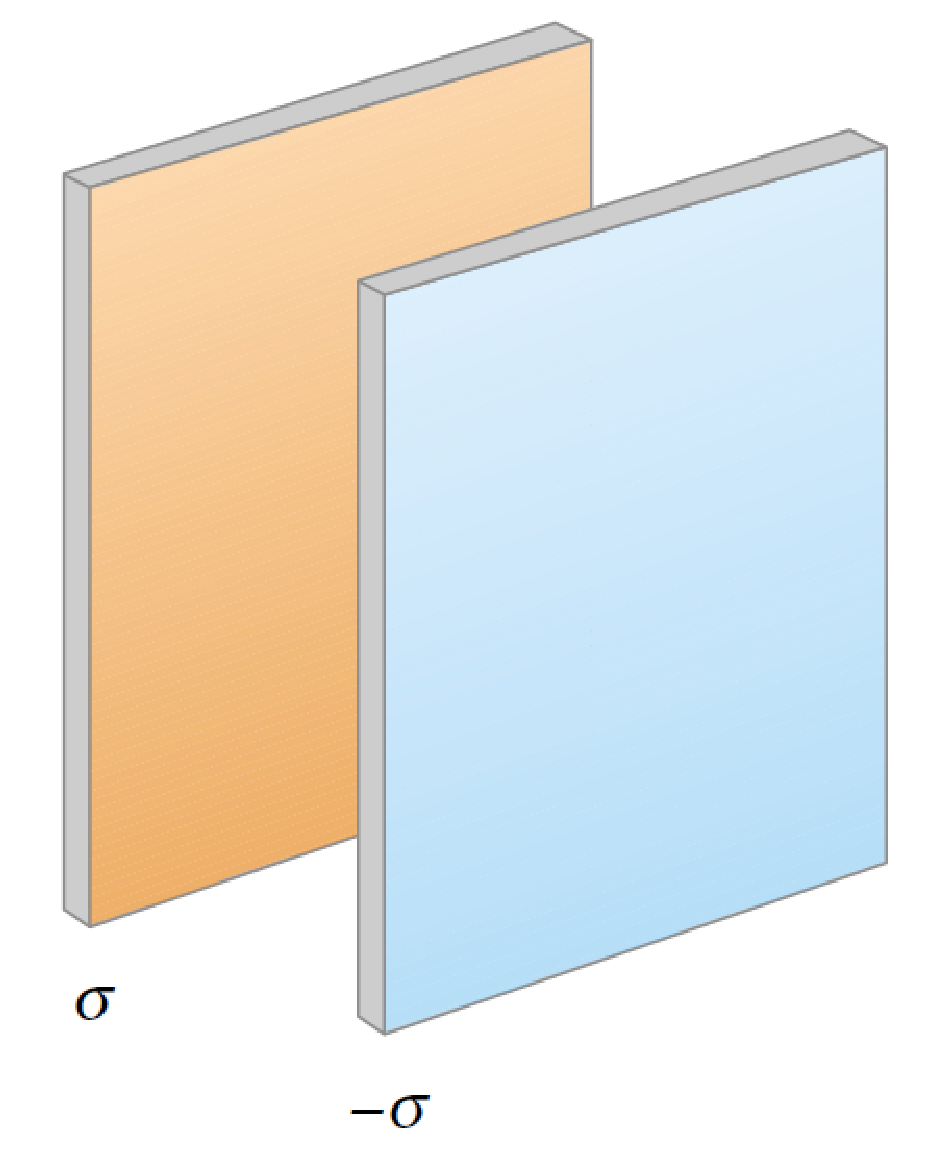
\includegraphics[scale=0.2]{placas-paralelas}
\end{center}
}
\begin{displaymath}
E=\dfrac{\sigma}{\epsilon_{0}} \hspace{0.3 cm} (\text{interior}) \hspace{0.3 cm} E=0 \hspace{0.3 cm} (\text{exterior}).
\end{displaymath}

\end{enumerate}

\end{document}
